%----------------------------------------------------------------------------------------
%-----------------------------------Script Stuff-----------------------------------------
%----------------------------------------------------------------------------------------
% JAVASCRIPT

\lstdefinelanguage{JavaScript}{
  keywords={typeof, new, true, false, catch, function, return, null, catch, switch, var, if, in, while, do, else, case, break},
  keywordstyle=\color{blue}\bfseries,
  ndkeywords={class, export, boolean, throw, implements, import, this},
  ndkeywordstyle=\color{darkgray}\bfseries,
  identifierstyle=\color{black},
  sensitive=false,
  comment=[l]{//},
  morecomment=[s]{/*}{*/},
  commentstyle=\color{purple}\ttfamily,
  stringstyle=\color{red}\ttfamily,
  morestring=[b]',
  morestring=[b]"
}

\lstset{
   language=JavaScript,
   backgroundcolor=\color{lightgray},
   extendedchars=true,
   basicstyle=\footnotesize\ttfamily,
   showstringspaces=false,
   showspaces=false,
   numbers=left,
   numberstyle=\footnotesize,
   numbersep=9pt,
   tabsize=2,
   breaklines=true,
   showtabs=false,
   captionpos=b
}

% PYTHON 
% Python style for highlighting
\newcommand\pythonstyle{\lstset{
language=Python,
basicstyle=\ttm,
otherkeywords={self},             % Add keywords here
keywordstyle=\ttb\color{deepblue},
emph={MyClass,__init__},          % Custom highlighting
emphstyle=\ttb\color{deepred},    % Custom highlighting style
stringstyle=\color{deepgreen},
frame=tb,                         % Any extra options here
showstringspaces=false            % 
}}


% Python environment
\lstnewenvironment{python}[1][]
{
\pythonstyle
\lstset{#1}
}
{}

% Python for external files
\newcommand\pythonexternal[2][]{{
\pythonstyle
\lstinputlisting[#1]{#2}}}

% Python for inline
\newcommand\pythoninline[1]{{\pythonstyle\lstinline!#1!}}
%----------------------------------------------------------------------------------------

\chapter{System Design}

\begin{figure}[H]
	\caption{Final System Architecture}
	\label{image:design}
	\centering
	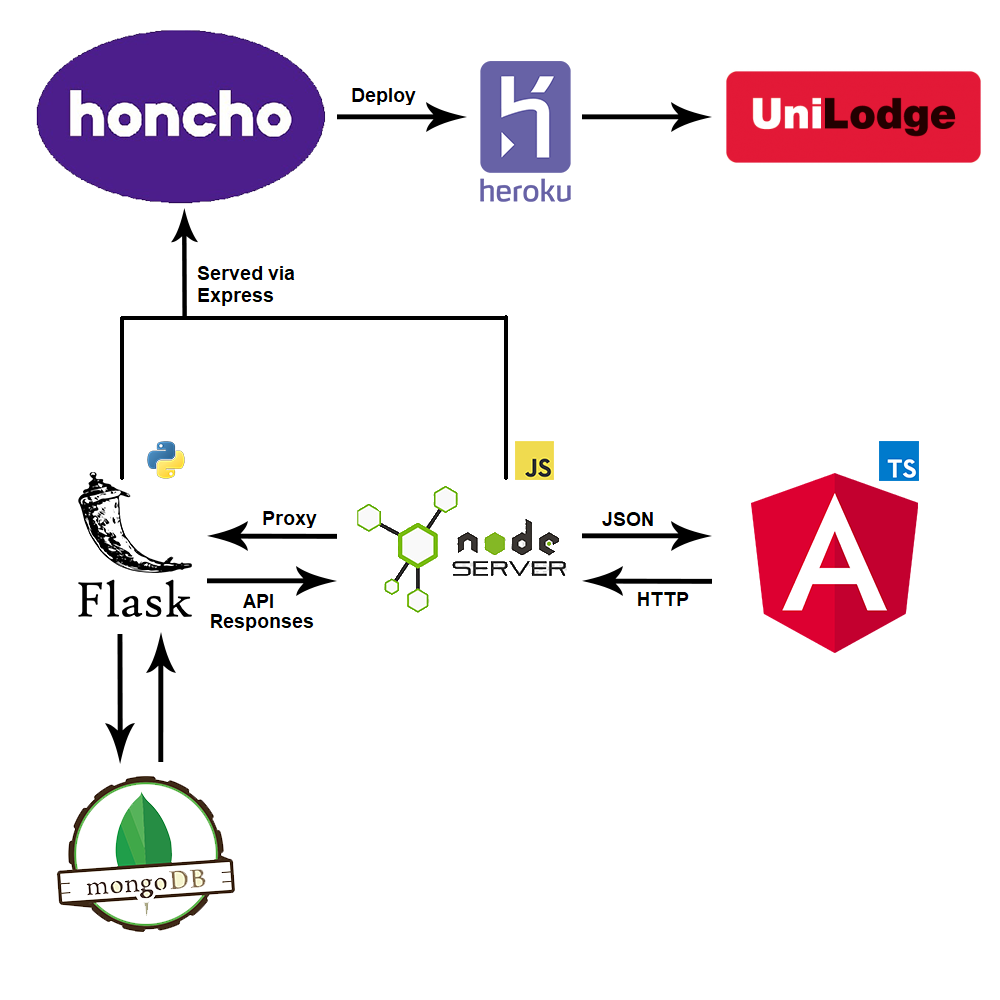
\includegraphics[width=1\textwidth]{images/design.png}
\end{figure}	

\section{Architectural Overview}
The overall design of the system changed at multiple points throughout the development cycle before arriving at the conclusive design that can be seen in \textbf{Fig.\ref{image:design}}. This section will give a brief high-level overview of how the final architectural design came to be.

\subsection{Major Architectural Changes}
Initially, the project during development consisted of Angular for the presentation layer, Flask for the server and MongoDB Atlas for the database. Routes would be defined with Angular and API calls would be directed towards Flask which would in turn interact with MongoDB Atlas and return a response to the frontend.

\paragraph{}
During deployment however a major shift in design occurred. Major issues were encountered whenever Heorku used Flask to serve static Angular build files, resulting in pages and components not working as they would locally. To address this, Node and Express were used to serve the Angular build files. A server proxy would redirect Express API calls to the Flask server address, allowing Flask to retain it's role as the sole API while using the Express server to serve the Angular build files. This action, while somewhat convoluted, did address the issue which had caused a blocker for multiple days.

\subsection{Final Architectural Design}
The conclusive design (\textit{Which can be seen in \textbf{Fig.\ref{image:design}}}) allows the overall system to be delivered to users via cloud services, enabling a software as a service distribution model. 

\paragraph{}
A Honcho procfile is used to enable the execution of both the Flask API server and the Express/Node server using just one worker on the cloud. Heroku will use Express/Node to serve the Angular build files while RESTful requests made to the Express server will be redirected to Flask with the use of a server proxy, allowing interactions between the primary components of the system to remain unhindered.

\paragraph{}
Further insight on the decisions made during the development cycle and how the overall system is structured, including how individual components interact with each other will be discussed throughout the chapter.\newline

\section{Data Tier}
MongoDB Atlas was employed to manage all the data-related needs of the project. Database operations are all executed by Python, based on requests made to the API by the frontend. In this section, the interactions between the aforementioned data related components will be conveyed and their inner-workings explained.

\subsection{Database Models}
Models had to be defined to represent intractable entities within the system. These models can be interacted with allowing an array of CRUD functionality. Key values were used to associate associative models, enabling the simplification of the overall cluster and allow for the employment of functions like cascading operations.

\begin{lstlisting}[caption=Definiton of Database Models]
export class Listing { 
    public Unique_Id: any,
    public Title: string,
    public Seller: string,
    public Description: any,
    public Location: any,
    public Price: number,
    public ContactNumber: string,
    public Image?: string,
}
export class User { 
  _id: number;
  Username: string;
  Password: string;
  Image?: any;
}
export class Comment { 
    Listing_ID: string;
    Comment_ID: any;
    Poster: string;
    Content: string;
    Timestamp?: any;
 }
\end{lstlisting}

The models were defined at a class level, permitting more control and allowing the ability to define an attribute as optional or required. With TypeScript, this was accomplished by appending a '\textbf{?}' to the name of the attribute, defining it as an optional value.

\paragraph{}
Unique values were used to associate key values to associative models, all content created by a specific user will always be associated with that user's unique ID, making operations like finding all comments or posts by that user a simplified task.

\subsection{MongoDB Atlas Interactions}
The Python library \textbf{PyMongo} was utilized to expose and allow for the use of the full suite of Mongo utility methods and crucial CRUD commands. 

\paragraph{}
To adhere to the single responsibility principle, a specific Python class was constructed that would encapsulate the accession of specific data collections. For each collection, a method would be defined, permitting invocation of the method which will return the collection object which can be used for manipulation. \newline

\begin{python}[caption=Database Accession Class]
from flask_pymongo import MongoClient

# URI for database connection was stored in a local file for security
with open("mongo_uri.txt", "r") as uri:
    MONGO_URI = uri.read()
    
cluster = MongoClient(MONGO_URI)
database = cluster["UniLodge"]

def Users():
    users = database["Users"]
    return users
\end{python}

Based on the defined class in \textbf{Listing.4.2}, the collections could be called externally, enabling encapsulation of the collection logic while still exposing necessary PyMongo functionality. In classes that would externally interact with the collections, the manipulation of collections would still be simplistic, they would need only to import and define the accession class. \newline

\begin{python}[caption=Interacting with Collections]
# Definition of Database class as d_a
import data.database_accessor as d_a

@temp_users_blueprint.route('/api/users', methods=['GET'])
def list_users():
    # The object d_a allows full control of the collection
    userList = list(d_a.Users().find({}, {'_id': False}))

    return jsonify(userList)
\end{python}

As can be seen in \textbf{Listing.4.3}, interactions with the collection objects still remain practical and simplistic. In this specific scenario, a list of users are returned to the client as a JSON object, enabling further interaction with the collection by the client.

\subsection{Hashing}
To ensure sensitive user information would never be compromised, the Python library Bcrypt was employed in the backend, allowing the encryption of confidential data. \newline

\begin{python}[caption=Hashing a Password with Bcrypt]
import bcrypt as bc

def generate_hash(plain_text_password):
    pw_hash = bc.bcrypt.hashpw(plain_text_password.encode("utf-8"), bc.gensalt())
    return pw_hash
\end{python}

\paragraph{}
The function defined in \textbf{Listing.4.1} when provided with a plain text password, generates a salted hash and returns the hashed password to the caller. The function is called whenever a newly registered user submits a registration form with their plain-text password being the sole parameter for the function. Once called, the plain-text password is hashed and salted, before being stored in the database as the designated hash. \newline

\begin{python}[caption=Verifing a Password]
import bcrypt as bc

def check_password(plain_text_password, hashed_password):
    if bc.bcrypt.checkpw(plain_text_password, hashed_password):
        result = True
    else:
        result = False # Password is wrong :(
    return result
\end{python}

The hashing algorithm used is one-way, meaning it can never be decrypted back to it's original plain text password. To verify the user in the future if for example they want to login, when their plain text password is entered it will again be hashed, this new hash will be compared against the hash stored in the database from when they previously registered. Should both hashes match, it would prove the passwords are the same considering the same input will always yield the same hash.

\section{Logic Tier}
The middle tier for the system acts as a doorway between the data tier and presentation tier. This tier consists of a mix of Python and TypeScript. API requests defined in TypeScript service files are propagated to the Flask API, depending on the undertaken user action. The API performs performs an action, generally in relation to the database and propagates a response back to the user through the TypeScript service file. This section will break down and further explain the interlinked processes that make up this tier.

\subsection{Flask API}
The API is completely written with Flask and documented with Swagger. TypeScript handles the sending of requests to the API. Simplistic methods contain the API endpoint to invoke as well as the expected object that should be return.

\begin{lstlisting}[caption=Basic Request to the API]
getListings(): Observable<Listing[]> {
  return this.http.get<Listing[]>(this.userUrl + '/api/listings');
}
\end{lstlisting}

The TypeScript method in \textbf{Listing 4.6} will seek the it's defined API endpoint and will expect an array of Listings. Assuming the Flask server is running, the endpoint will be accessed and will return a Listings array for use in the frontend. \newline

\begin{python}[caption=API Counterpart Route]
@listings.route('/api/listings', methods=['GET'])
def list_listings():
    # Find all listings within the Database
    listings = list(d_a.Listings().find({}, {'_id': False}))
    
    # Send the list of listings to the frontend
    return jsonify(listings)
\end{python}

\subsubsection{Blueprint}
Using the Python library \textbf{Blueprint}, routes could be categorized and coupled together in separate classes depending on their function. This allowed a single class to handle all requests and delegate a task to it's designated route and class. \newline

\begin{python}[caption=Main Flask Runner]
from routes.login_route import login_blueprint 
from routes.register_route import register_blueprint
from routes.temp_users_route import temp_users_blueprint
from routes.listings_route import listings_blueprint

app.register_blueprint(login_blueprint) 
app.register_blueprint(register_blueprint)
app.register_blueprint(users_blueprint)
app.register_blueprint(listings_blueprint)

if __name__ == "__main__":
    app.run() 
\end{python}

\subsubsection{API Documentation}
The view the full API documentation via Swagger, see \textit{Appendices}. 

\subsection{Authentication}
To further secure and authenticate the overall system, JSON Web Tokens were employed with the help of the Python library Flask\_JWT, which would only allow the accession of sensitive routes if the user had a specific access token saved in their local browser storage. The token will be stored locally whenever a login is successful, allowing the navigation of sensitive routes.  \newline

\begin{python}[caption=Issuing a limited JWT Token ]
from flask_jwt_extended import JWTManager

# Load confidential Secret Key from local file
app.config.from_envvar('SECRET_KEY')

jwt = JWTManager(app)

@login.route('/api/login', methods=['POST'])
def login():
    if (p_h.check_password(password, stored_hash)): 
        # Map JWT token to the Username
        # Set it to expire in 25 minutes
        result = create_access_token(identity=str(username), expires_delta=(datetime.timedelta(minutes=25)))
    else:
        result = Invalid
    return jsonify(result)
\end{python}

\newpage
Following the issuing of the token, the now authenticated user may access routes that previously locked. This is accomplished with a simple method decorator (\textbf{@token\_required}) as well as some TypeScript logic. \newline

\begin{python}[caption=Issuing a limited JWT Token]
# Create a new Listing
@listings_blueprint.route('/api/new-listing/<string:Username>', methods=['POST'])
@token_required
def new_listing(Username):
    Username = get_jwt_identity()
    listing_data = json.loads(request.get_data().decode())
   
    try: 
        d_a.Listings().insert_one(listing_data) 
        result = Success
    except:
        result = Invalid
    
    return jsonify(result)
\end{python}



\subsection{Angular Routing}

\section{Application Tier}
\subsection{Pages?}
\subsection{Styling?}
\subsection{Deployment}